% $Id: template.tex 11 2007-04-03 22:25:53Z jpeltier $

\documentclass{vgtc}                          % final (conference style)
%\documentclass[review]{vgtc}                 % review
%\documentclass[widereview]{vgtc}             % wide-spaced review
%\documentclass[preprint]{vgtc}               % preprint
%\documentclass[electronic]{vgtc}             % electronic version

%% Uncomment one of the lines above depending on where your paper is
%% in the conference process. ``review'' and ``widereview'' are for review
%% submission, ``preprint'' is for pre-publication, and the final version
%% doesn't use a specific qualifier. Further, ``electronic'' includes
%% hyperreferences for more convenient online viewing.

%% Please use one of the ``review'' options in combination with the
%% assigned online id (see below) ONLY if your paper uses a double blind
%% review process. Some conferences, like IEEE Vis and InfoVis, have NOT
%% in the past.

%% Figures should be in CMYK or Grey scale format, otherwise, colour 
%% shifting may occur during the printing process.

%% These few lines make a distinction between latex and pdflatex calls and they
%% bring in essential packages for graphics and font handling.
%% Note that due to the \DeclareGraphicsExtensions{} call it is no longer necessary
%% to provide the the path and extension of a graphics file:
%% \includegraphics{diamondrule} is completely sufficient.
%%
\ifpdf%                                % if we use pdflatex
  \pdfoutput=1\relax                   % create PDFs from pdfLaTeX
  \pdfcompresslevel=9                  % PDF Compression
  \pdfoptionpdfminorversion=7          % create PDF 1.7
  \ExecuteOptions{pdftex}
  \usepackage{graphicx}                % allow us to embed graphics files
  \DeclareGraphicsExtensions{.pdf,.png,.jpg,.jpeg} % for pdflatex we expect .pdf, .png, or .jpg files
\else%                                 % else we use pure latex
  \ExecuteOptions{dvips}
  \usepackage{graphicx}                % allow us to embed graphics files
  \DeclareGraphicsExtensions{.eps}     % for pure latex we expect eps files
\fi%

%% it is recomended to use ``\autoref{sec:bla}'' instead of ``Fig.~\ref{sec:bla}''
\graphicspath{{figures/}{pictures/}{images/}{./}} % where to search for the images
\usepackage{listings}
\usepackage{microtype}                 % use micro-typography (slightly more compact, better to read)
\PassOptionsToPackage{warn}{textcomp}  % to address font issues with \textrightarrow
\usepackage{textcomp}                  % use better special symbols
\usepackage{mathptmx}                  % use matching math font
\usepackage{times}                     % we use Times as the main font
\renewcommand*\ttdefault{txtt}         % a nicer typewriter font
\usepackage{cite}                      % needed to automatically sort the references
\usepackage{tabu}                      % only used for the table example
\usepackage{booktabs}                  % only used for the table example
%% We encourage the use of mathptmx for consistent usage of times font
%% throughout the proceedings. However, if you encounter conflicts
%% with other math-related packages, you may want to disable it.


%% If you are submitting a paper to a conference for review with a double
%% blind reviewing process, please replace the value ``0'' below with your
%% OnlineID. Otherwise, you may safely leave it at ``0''.
\onlineid{0}

%% declare the category of your paper, only shown in review mode
\vgtccategory{Research}

%% allow for this line if you want the electronic option to work properly
\vgtcinsertpkg

%% In preprint mode you may define your own headline.
%\preprinttext{To appear in an IEEE VGTC sponsored conference.}
\usepackage{color}
\definecolor{lightgray}{rgb}{.95,.95,.95}
\definecolor{darkgray}{rgb}{.4,.4,.4}
\definecolor{purple}{rgb}{0.65, 0.12, 0.82}

\lstdefinelanguage{JavaScript}{
  keywords={typeof, new, true, false, catch, function, return, null, catch, switch, var, if, in, while, do, else, case, break},
  keywordstyle=\color{blue}\bfseries,
  ndkeywords={class, export, boolean, throw, implements, import, this},
  ndkeywordstyle=\color{darkgray}\bfseries,
  identifierstyle=\color{black},
  sensitive=false,
  comment=[l]{//},
  morecomment=[s]{/*}{*/},
  commentstyle=\color{purple}\ttfamily,
  stringstyle=\color{red}\ttfamily,
  morestring=[b]',
  morestring=[b]"
}

\lstset{
   language=JavaScript,
   backgroundcolor=\color{lightgray},
   extendedchars=true,
   basicstyle=\footnotesize\ttfamily,
   showstringspaces=false,
   showspaces=false,
   numbers=left,
   numberstyle=\footnotesize,
   numbersep=9pt,
   tabsize=2,
   breaklines=true,
   showtabs=false,
   captionpos=b
}
%% Paper title.

\title{\"Uberarbeitung wissenschaftlicher Arbeiten anhand einer Kombination von Text Mining und Visualistik}


%% Author and Affiliation (multiple authors with multiple affiliations)
\author{Sascha Lemke\\ %
        \scriptsize Matr.Nr.: 11074933 %
\and Dennis Dubbert\\ %
     \scriptsize Matr.Nr.: 11089478}

%% A teaser figure can be included as follows, but is not recommended since
%% the space is now taken up by a full width abstract.
%\teaser{
%  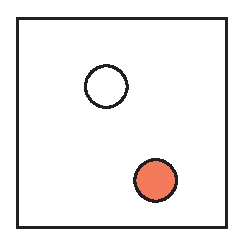
\includegraphics[width=1.5in]{sample.eps}
%  \caption{Lookit! Lookit!}
%}

%% Abstract section.
\abstract{Duis autem vel eum iriure dolor in hendrerit in vulputate
velit esse molestie consequat, vel illum dolore eu feugiat nulla
facilisis at vero eros et accumsan et iusto odio dignissim qui blandit
praesent luptatum zzril delenit augue duis dolore te feugait nulla
facilisi. Lorem ipsum dolor sit amet, consectetuer adipiscing elit,
sed diam nonummy nibh euismod tincidunt ut laoreet dolore magna
aliquam erat volutpat. Ut wisi enim ad minim veniam, quis nostrud exerci tation ullamcorper
suscipit lobortis nisl ut aliquip ex ea commodo consequat. Duis autem
vel eum iriure dolor in hendrerit in vulputate velit esse molestie
consequat, vel illum dolore eu feugiat nulla facilisis at vero eros et
accumsan et iusto odio dignissim qui blandit praesent luptatum zzril
delenit augue duis dolore te feugait nulla facilisi.%
} % end of abstract


\begin{document}

%% The ``\maketitle'' command must be the first command after the
%% ``\begin{document}'' command. It prepares and prints the title block.

%% the only exception to this rule is the \firstsection command
\firstsection{Einleitung}

\maketitle

%% Introduction starts here %%
In den letzten Jahren haben immer mehr digitale Medien Einzug in das alltägliche Leben gehalten. Insbesondere das Internet ist dabei für einen Großteil der Veränderung verantwortlich. Doch neben Bildern, Videos und Audio ist der Text, gerade auch durch das Internet, immer noch das wichtigste Kommunikationsmittel für Wissen.\\

Doch nicht nur im alltäglichen Leben, insbesondere im wissenschaftlichen Umfeld ist Schrift und Sprache wichtig. Das Verfassen von Hausarbeiten oder das spätere Schreiben von Artikeln für Journale erfordert dabei ein gewisses Maß an Qualität. Diese Qualität wird oft durch Erfahrung, einhalten von diversen Richtlinien und Zeit in Form von wiederholten Iterationen erreicht.\\

Dieses Projekt versucht diesen Prozess mit Hilfe von Visualisierungen von Text Mining Daten zu unterstützen. In vielen Leitfäden zu wissenschaftlichem Schreiben finden sich Richtlinien wie Präzision oder das vermeiden von Wortwiederholungen. Diese Werte lassen sich mit Text Mining und Mitteln der deskriptiven Statistik leicht ermitteln und dienen als Grundlage für die in diesem Dokument beschriebenen Visualisierungen. Aus diesem Grund sollten die Texte auf folgende Eigenschaften untersucht werden:\\

\begin{itemize}
\item Worthäufigkeit (Redundanz)
\item Satzlänge (Komplexität)
\item Satzzeichen (Komplexität)
\item Füllwörter (Präzision)
\end{itemize}

Im folgenden Kapitel wird beschrieben, welche Text Mining Verfahren eingesetzt wurden, um die Daten für die Visualisierung der oben beschrieben Eigenschaften zu gewinnen.

\section{Text Mining und Datenstrukturen}
Um die oben beschrieben Eigenschaften visualisieren zu können muss eine entsprechende Datenbasis geschaffen werden, welches durch Text Mining ermöglicht wird. Der Prozess teilt sich dabei in folgende Schritte auf:

\begin{itemize}
\item Aufgabendefinition
\item Dokumentselektion
\item Dokumentaufbereitung
\item (Text) Mining Methoden
\item Interpretation / Evaluation
\item Anwendung
\end{itemize}

Die in der Einleitung beschrieben Motivation bildet die Aufgabendefinition dieses Projekts. Der nächste Schritt umfasst die Recherche und Sammlung von Dokumenten, welche dem Erreichen der vorher formulierten Ziele der Aufgabendefinition dienen. Oft werden dabei Dokumente aus verschiedenen Quellen mit verschiedenen Formaten entnommen.  Die Aufbereitung der Dokumente nimmt in einem Text Mining Vorhaben den größten Zeitaufwand ein, da hier Formate, Codierungen und Zeichen standardisiert werden müssen. Vor der Anwendung der Ergebnisse müssen die Daten noch interpretiert und evaluiert werden. Dabei kommen oft Experten mit entsprechenden Domänenwissen zum Einsatz, denn auch heute noch kommt Text Mining nicht komplett ohne menschliche Komponenten aus.

\subsection{Vorverarbeitung}
Da sich dieses Projekt primär auf die Visualisierung der Daten konzentriert wurde die Menge der Dokumente begrenzt und die die Vorverarbeitung entsprechend angepasst um zu Zeit sparen. \\

Hierbei wurde aus Zeitgründen nur ein Dokument gewählt, welches die Möglichkeiten von Text Minung und Visualisierung verdeutlichen soll. Dieses wurde entsprechend mit Hilfe von XML standardisiert. So fällt ein Großteil der Zeit für die Sammlung von Dokumenten und dessen Standardisierung weg, welche in für die Visualisierung genutzt werden kann. \\

Durch diese Standardisierung lässt sich das Dokument nun auf mehreren Ebenen analysieren.

\subsubsection{Morphologisch}
Die morphologische Untersuchung behandelt die Texte auf Zeichenebene. Dabei werden folgende Verfahren auf Wortformen (sogenannte Token) angewendet. Hier einige Beispiele:\\

\begin{itemize}
\item Tokenisierung
\item Finden von Satzenden
\item Stammformreduktion (Stemming)
\end{itemize}

Üblicherweise beginnt man damit den Text in einzelne Wortformen (Token) zu zerlegen. Dabei wird in westlichen Sprachen üblicherweise das "white-space-tokenizing" verwendet. Dabei werden Strings anhand von Leerzeichen, Tabs, Zeilenumbrüchen und ähnlichen Trennzeichen aufgetrennt. Dabei treten erste Probleme auf, da nicht jede Sprache über Leerzeichen verfügt (Chinesisch) oder Wörter wie "New York" werden als einzelne Worte betrachtet, obwohl sie zusammen gehören.\\

Der nächste Schritt umfasst das Finden von Satzgrenzen. Auch hier treten einige Herausforderungen auf, da beispielsweise nicht jeder Punkt ein Satzende darstellt. So bilden Abkürzungen wie "Dr." oder "et al." keine Satzgrenzen und müssen daher entsprechend dem Token zugeordnet werden.\\

Ein weiterer Schritt ist das Stemming, welcher allerdings oft in Abhängigkeit der Text Mining Ziele durchgeführt wird. So gibt es hier einfache Normalisierungen wie das Auflösen von Ein- und Mehrzahl, welches man auch als "Inflectional Stemming" bezeichnet. Das Ziel dabei ist es die Genauigkeit der folgenden Analyse zu erhöhen, etwa bei statistischen Analysen wie Worthäufigkeiten. Als Gegensatz dazu existiert auch das "Root Stemming", welches eine aggressivere Form des Stemmings darstellt. Dabei geht das Stemming so weit, das Token wie "Application" auf ihren eigentlichen Wortstamm zurückgeführt werden ("apply").\\

Da diese Untersuchungen oft die Grundlage von Text Mining Vorhaben bilden werden auch in diesem Projekt einige der oben genannten Methoden verwendet. So wurden die Texte tokenisiert und die Satzgrenzen entsprechend gekennzeichnet. \\

Durch die Tokenisierung des Dokuments lassen sich die notwendigen Worthäufigkeiten (genauer: Token)  für die Visualisierung ermitteln. Zusätzlich kann dadurch die Satzlänge und die das Auftreten von Satzzeichen ermittelt werden, was die Daten für die Ermittlung der oben beschriebenen Komplexität liefert.

\subsubsection{Syntaktisch}

Die syntaktische Ebene befasst sich mit der Untersuchung von Texten auf Satzebene. Dabei werden die Zeichen in Beziehung zueinander gestellt und untersucht. Beispiele dafür sind folgende:\\

\begin{itemize}
\item Part-of-Speech
\item Phrase Recognition
\end{itemize}

Bei dem Part-of-Speech Tagging handelt es sich um das Erkennen von Wortklassen (Nomen, Verben, ...) und die Annotation der Token mit selbigen. Aufgrund der Vielfältigkeit von Sprache (und dem Umstand das eine Sprache lebt) werden hier oft statistische Ansätze verwendet. 

Bei der Phrase Recognition geht es darum Phrasen in Texten zu erkennen. So können POS-Tags dabei helfen bestimmte Wortgruppen zu finden, oder einfache Form wie das "Noun phrase chunking" ermöglichen.\\

Wie bereits oben beschrieben liegt der Fokus auf diversen Messwerten, daher ist eine syntaktische Untersuchung der Texte in diesem Projekt nicht zielführend. Dennoch wurden mit Hilfe von Part-of-Speech Tagging versucht Werte für eine mögliche Erkennung des Nominalstils zu sammeln, welche im Ausblick diskutiert werden.

\subsubsection{Semantisch}
Die semantische Analyse befasst sich mit der Bedeutung von Wörtern und ihrer digitalen Darstellung. Hier wird oft auf Hintergrundwissen zurück gegriffen, so werden beispielsweise Fachsprachen (Informatik, Medizin, etc) über Ontologien oder Taxonomien modelliert und in den Prozess eingebunden. Damit sollen Probleme wie beispielsweise Mehrdeutigkeit (Word Sense Disambiguation) umgangen werden. \\

Diese Art der Untersuchung erfordert allerdings einen größeren Umfang, als es in diesem Projekt möglich war, daher wurden keine semantischen Untersuchungen durchgeführt.

\subsection{Analyse}
Der Bereich Text und Data Mining umfasst eine große Mengen an Methoden um diverse Informationen aus Texten zu extrahieren bzw zugänglich zu machen. So werden diese oft in verschiedene Kategorien eingeteilt, wie beispielsweise das Information Retrieval oder Information Extraction. Diese Methoden sind sehr weitreichend und aufwendig. Eine entsprechende Vorstellung und Durchführung sind nicht Ziel dieses Projekts, daher wird an dieser Stelle darauf verzichtet.\\

Stattdessen werden statistische Hilfsmittel genutzt um Daten für die Visualisierungen zu gewinnen. Dabei werden Mittel der deskriptiven Statistik verwendet um die in der Einleitung beschrieben Werte zu ermitteln.

So ist insbesondere die Häufigkeit diverser Token ein wichtiger Messwert, welcher als Grundlage für eine qualitative Aussage dienen soll. Dabei handelt es sich um folgende einfache Formel:

$ tf(t,d) = f_{t,d} $

Dabei beschreibt $t$ den Term und und $d$ das Dokument. Da hier nur ein Dokument als Grundlage dient handelt es um eine einfache Summenfunktion:

$\sum_{i=1}^{n} t_i$

Neben diesen Recht einfachen Werten sollen zusätzliche statistische Werte einen Überblick geben. So sollen Median und Durchschnitt zusätzliche Informationen anbieten, beispielsweise ein die durchschnittliche Satzlänge oder Verwendung von Satzzeichen.

\subsection{Datenstruktur und Implementierung}
Da die Visualisierung mit Hilfe von d3.js implementiert wird, werden die Daten in JSON bereitgestellt. Die Texte werden mit Hilfe von Open NLP der Apache Software Foundation aufbereitet, welches Java als Programmiersprache nutzt. Da das Dokument bereits in XML standardisiert ist, lässt es sich leicht mit Hilfe von JAXB und Data Binding in Java Objekte übersetzen. \\

Open NLP stellt außerdem einige Modelle bereit um Aufgaben wie Tokenisierung oder Part-of-Speech Tagging durchzuführen. Die Daten werden im Anschluss mit einem Node.js Server gekoppelt um diverse Filteroptionen zu ermöglichen.\\

In den folgenden Abschnitten werden die gesammelten Daten und deren Datenstrukturen im Detail beschrieben.

\subsubsection*{Worthäufigkeit}
Die Worthäufigkeit wird durch durch ein Schlüssel-Wert-Paar dargestellt und mit Informationen über den Fundort angereichert. So wird nicht nur das Wort und die Anzahl gespeichert, sondern das Kapitel und die entsprechenden Unterkapitel mit gespeichert. Zusätzlich wurde der Wert in Abhängigkeit der gesamten Wortanzahl des Fundorts normalisiert. Daraus ergibt sich folgende Datenstruktur:

\begin{lstlisting}
{
  "word" : "visualization",
  "count" : 1,
  "chapterID" : 1,
  "sectionID" : 2,
  "subsectionID" : 0,
  "subsubsectionID" : 0,
  "normalized" : 0.4484304932735426
}
\end{lstlisting}

\subsubsection*{Satzlänge}
Die Sätzlänge wird ebenfalls durch die Häufigkeit dargestellt und mit ID's versehen. Hier erhält zusätzlich jeder Satz noch eine eigene ID und der Satz wird im Original mit gespeichert.

\begin{lstlisting}
{
  "chapterID" : 1,
  "sectionID" : 2,
  "subsectionID" : 0,
  "subsubsectionID" : 0,
  "sentenceID" : 135,
  "length" : 17,
  "sentence" : "Visual analytics (VA) is typically applied in scenarios where complex data has to be analyzed."
}
\end{lstlisting}

\subsubsection*{Satzzeichen}
Die Struktur Satzzeichen ist an der Struktur der Sätzlänge angelehnt. Der wichtige Unterschied ist das hier eine Liste der Position der Token mit angegeben wird um im Nachhinein zu aufzuzeigen, an welcher Stelle sich die Satzzeichen befinden.

\begin{lstlisting}
{
  "sentenceID" : 135,
  "count" : 2,
  "sentence" : "Visual analytics (VA) is typically applied in scenarios where complex data has to be analyzed.",
  "token" : [ 4, 17 ],
  "chapterID" : 1,
  "sectionID" : 2,
  "subsectionID" : 0,
  "subsubsectionID" : 0
}
\end{lstlisting}

\subsubsection*{Füllwörter}
Da die Füllwörter nicht durch einen einfachen Zähler dargestellt werden können unterscheidet sich diese Datenstruktur stark von den bisher vorgestellten. Da die Füllwörter pro Paragraph berechnet wurden erscheint hier eine zusätzliche ID. Auch eine Liste der Token ID's wurde übernommen, um die Position der Füllwörter aufzuzeigen. Da Paragraphen weder durch Text noch durch Zahlen eindeutig zu beschreiben sind werden hier auch die Titel der diversen Überschriften mit angegeben um so eine verständliche Zuordnung zu ermöglichen. 

\begin{lstlisting}
{
  "paragraphID" : 3,
  "count" : 94,
  "token" : [ 5, 8, 10, 13, 14, 15, 20, 21, 22, 25, 26, 28, 29, 31, 32, 34, 35, 37, 39, 44, 47, 48, 51, 52, 54, 59, 62, 65, 67, 70, 71, 77, 79, 81, 82, 85, 86, 87, 89, 90, 92, 95, 100, 101, 103, 108, 110, 111, 114, 118, 120, 121, 123, 126, 128, 132, 133, 142, 143, 145, 146, 148, 150, 152, 154, 156, 159, 164, 168, 169, 171, 173, 176, 177, 181, 184, 188, 191, 196, 197, 198, 199, 200, 201, 203, 205, 206, 207, 208, 211, 214, 218, 219, 221 ],
  "chapterID" : 1,
  "sectionID" : 2,
  "subsectionID" : 0,
  "subsubsectionID" : 0,
  "chaptername" : "abstract",
  "sectionname" : null,
  "subsectionname" : null,
  "subsubsectionname" : null,
  "idInChapter" : 1
}
\end{lstlisting}
\section{Aufbau der Visualisierung}
Die Visualisierung ist in zwei Abschnitte eingeteilt, welche vertikal voneinander Abgetrennt sind und in einer starken Synergie stehen. Die Linke Seite des Bildschirms wird von der eigentlichen Visualisierung eingenommen und die rechte Seite stellt einen Text-View dar. In der Visualisierung k\"onnen verschiedenen Auswahlen getroffen und hierdurch innerhalb des Text-Views markiert werden. Anhand der textuellen Darstellung und N\"ahe der markierten Begriffe kann der Nutzer nun R\"uckschl\"usse bez\"uglich der Wissenschaftlichkeit seines Dokuments bilden und gegebenenfalls Verbesserungen an diesem vornehmen. Die Abschnitte sind durch einen Balken klar abgetrennt, welcher jedoch, jeh nach Anforderung des Nutzers, verschoben werden kann, um die Gr\"o{\ss}enverh\"altnisse anzupassen. Wird gerade eine Auswahl getroffen, so kann es n\"tzlich sein die Visualisierungsseite zu vergr\"o{\ss}ern. Wurde bereits eine Auswahl getroffen so kann die Textseite verg\"o{\ss}ert werden.\\
Um eine geeignete und feingranulare Auswahl dieser Begriffe gew\"ahrleisten zu k\"onnen, ist auch der Visualisierungsbereich in weitere, aufeinander aufbauende, Einzelvisualisierungen gegliedert. Somit beinhaltet sie:
\begin{center} 
   \begin{varwidth}{2in} 
      \begin{itemize} 
         \item eine Navigation,
		 \item eine Kapitel\"ubersicht / -auswahl,
		 \item und eine Detailansicht der Selektion 
      \end{itemize} 
   \end{varwidth} 
\end{center} 
Jede dieser Visualisierung hat ein festes Seitenverh\"altnis, sodass eine Verzerrung durch Gr\"o{\ss}en\"anderungen vermieden wird.\\
\\
Innerhalb der Navigation werden dem Nutzer zwei Drop-Down-Men\"us geboten, \"uber welche dieser die Visualisierungen an seine Anspr\"uche anpassen kann. Das erste dieser Men\"us erm\"oglicht ihm die Auswahl des gew\"unschten Testdokuments, \"uber das zweite Men\"u l\"asst sich die Filterungsmethode definieren (Redundanzen, Satzzeichen, Satzl\"ange oder F\"ullw\"orter). Wurde hier eine Auswahl getroffen, so wird die gesamte Visualisierung auf diese abgestimmt.\\
\\
Der zweite Abschnitt veranschaulicht die Hierarchie des ausgew\"ahlten Dokuments und wird f\"ur die Auswahl zu betrachtender Kapitel genutzt. Hier werden zwei alternative Ansichten geboten, eine in Form eines Sunburst und eine als Baumstruktur, welche teilweise unterschiedliche Auspr\"agungen hervorheben und sich somit gegenseitig erg\"anzen. \"Uber Tabs kann der Nutzer zu jedem Zeitpunkt die f\"ur ihn n\"utzlichere Ansicht selektieren. Wichtig ist hierbei, dass die, in den Ansichten get\"atigten, Auswahlen synchronisiert werden, wodurch ein flie{\ss}ender Wechsel unterst\"utzt wird. \\
\\
Wurde in der Kapitel\"ubersicht eine Auswahl getroffen, so wird diese in einer Detailansicht aufgegriffen. Hier sind die Begriffe der Ausgew\"ahlten Kapitel anhand der Filterungsmethode eingegrenzt und in Form eines Blasen-Diagramms visualisiert. Wurden beispielsweise Redundanzen selektiert, so steht jede Blase f\"ur ein Wort, welches innerhalb der Kapitelauswahl redundant auftritt. Zu jedem dieser Begriffe wird auch die entsprechende Auspr\"agung der Filterungsmethode bereitgestellt, sodass eine pers\"ohnliche Problemeinsch\"atzung des Nutzers erfolgen kann. Ist nun eine \"Uberarbeitung bestimmter Begriffe gew\"unscht, so k\"onnen diese selektiert und hierdurch jedes Vorkommnis, begrenzt durch die ausgew\"ahlten Kapitel, in dem Text-View markiert werden.\\
\\
Das folgende Kapitel dient somit zun\"achst der Erl\"auterung dieser Einzelvisualisierungen. Hierbei werden besonders die Entscheidungsfindungen und Kompromisse beleuchtet, welche zu dem Aufbau und den Interaktionsm\"oglichkeiten der jeweiligen Visualisierung f\"uhrten.

\subsection{Kapitel\"ubersicht: Sunburst-Diagramm} \label{subsec:sunburst}
Dem Sunburst-Diagramm liegt der Gedanke zugrunde, dass der Nutzer den Aufbau des Dokuments bereits kennt, sich also im Vorhinein damit auseinander gesetzt hat und nun mithilfe der Visualisierung eine weitere Iteration vornehmen m\"ochte. Im Fokus steht hierbei die bereits gut bekannte Kapitelhierarchie zentriert und auf einen Blick sichtbar darzustellen und somit eine schnelle Navigation und Auswahl zu erm\"oglichen. Da bei solch einem Diagramm nahezu keine Freifl\"achen zwischen den Elementen gegeben sind, kann den Elementen selber weitaus mehr Fl\"ache zugeordnet werden ohne die \"Ubersichtlichkeit der Visualisierung zu gef\"ahrden. Dies f\"uhrt zu einer Maximierung der Datendichte. Die verf\"ugbare Visualisierungsfl\"ache wird also bestm\"oglich ausgenutzt, da Lediglich das Zentrum und die Ecken des Diagramms Freifl\"achen bilden, welche jedoch f\"ur Informationstexte nutzbar sind. Bei einer Verkleinerung des Diagramms sind einzelne Abschnitte somit trotzdem klar erkenn- und trennbar, sodass die Visualisierung problemlos auf unterschiedlichen Bildschirmgr\"o{\ss}en angezeigt und genutzt werden kann.\\
\\
Ein weiterer Beweggrund f\"ur diese Art der Darstellung war, dass dem Nutzer ein Auswahlmedium bereitgestellt werden soll, welches die Dokumenthierarchie sowie Kapitel-Abh\"angigkeiten veranschaulicht. Durch die Aufeinanderschichtung der unterschiedlichen Ringlagen dieser Diagrammart sind die genannten Abh\"angigkeiten schnell erkennbar. Es werden keine weiteren visuellen Mittel ben\"otigt um die Zugeh\"origkeit eines Kapitels zu verdeutlichen, da die Position der Elemente ausreichend Aufschluss hier\"uber bietet. Somit wird auch die Data-Ink-Ratio erh\"oht und Chartjunk vermieden. Der mittlere Kreis stellt hierbei das Dokument dar, welches zun\"achst von den Hauptkapiteln (Abstract, Einleitung, Hauptteil, Fazit, etc.) umringt wird. Die Gr\"o{\ss}e des jeweiligen Ringabschnitts, in Abh\"angigkeit des Radius, ist hierbei der prozentuelle Anteil des Kapitels im Verh\"altnis zum gesamten Dokument. Als Ma{\ss} gilt hier die Wortanzahl eines Kapitels, welche sich aus dem eigenen Inhalt, sowie dem Inhalt aller Unterkapitel erschlie{\ss}en l\"asst und anschlie{\ss}end auf den entsprechenden Teilwinkel des Kreises umgerechnet wird. Dieses Schemata erstreckt sich auch auf die Unterkapitel eines Abschnittes, welche jedoch nun ihr jeweiliges Elternkapitel als Maximum ansehen (sowohl deren radialen Abschnitt in der Visualisierung als auch deren Wortanzahl) und nicht das gesamte Dokument.\\
\\
Ein Vorteil der hierdurch entsteht ist, dass neben der sichtbaren Hierarchie auch ein Gr\"o{\ss}enverh\"altnis zum jeweiligen Oberkapitel ersichtlich wird. F\"ur wissenschaftliche Arbeiten bestehen h\"aufig formale Anforderungen, sodass auch die Gr\"o{\ss}e einzelner Kapitel vorgegeben sein kann. Somit k\"onnte es also n\"utzlich sein solche Verh\"altnisse aus der Visualisierung entnehmen zu k\"onnen. Hierbei wurde jedoch bedacht, dass Gr\"{\ss}enverh\"altnisse in Kreisdiagrammen tr\"ugen k\"onnen, da der radiale Abschnitt die Gr\"o{\ss}e eines Ringabschnitts definiert und somit \"au{\ss}ere Abschnitte aufgrund ihrer Fl\"ache automatisch gr\"o{\ss}er erscheinen als Innere (auch bekannt als Lie Factor oder L\"ugenfaktor). Da bei der \"Uberarbeitung eines wissenschaftlichen Textes jedoch vorwiegend das direkte Verh\"altniss eines Kapitels zu Nachbarkapiteln des selben Oberkapitels betrachtet wird, wurde dieser Aspekt im Kontext des Projektes als vernachl\"assigbar eingesch\"atzt. Im Sunburst-Diagramm besitzen zudem alle Lagen die selbe H\"ohe, sodass der Fl\"acheninhalt hier eine geringere Bedeutung als der dargestellte Radius besitzt und somit trotzdem eine akkurate visuelle Einsch\"atzung get\"atigt werden kann. Damit der eigene Textanteil eines Oberkapitels ebenfalls mit den Textanteilen der Unterkapitel verglichen werden kann, wurde entschieden auch diesen Anteil als Unterkapitel aufzulisten und ihn somit auf deren Ebene zu verschieben. Diese werden jedoch als Einleitung betitelt und somit durch ihre Namensgebung speziell gekennzeichnet, sodass die Zugeh\"origkeit bestehen bleibt. Dies ist jedoch nur ben\"otigt, wenn ein Kapitel weitere Kapitel umschlie{\ss}t. Ansonsten wird der Textinhalt weiterhin im eigenen Element dargestellt.\\
\\
Da in einem wissenschaftlichen Dokument jedes Kapitel eine Einleitung besitzen sollte und dieses nicht direkt aus der bisherigen Visualisierung hervorgeht, wurde zudem eine M\"oglichkeit gesucht, fehlenden Text aufzuzeigen. Sollte also ein Kapitel keinen eigenen Text beinhalten, so wird in der Mitte des zugeh\"horigen Elements ein schwarzer Kreis gezeichnet. Dieser nimmt wenig Platz ein, wodurch die Data-Ink-Ratio nahezu unbeschadet bleibt. Durch die nun entstandene Unregelm\"a{\ss}igkeit innerhalb der Visualierung ist er jedoch auf den ersten Blick klar erkennbar, sodass dem Nutzer das Problem direkt \"ubermittelt wird.\\
\\
Ein weiterer wichtiger Aspekt dieser Visualisierung findet sich in der Farbgebung der Abschnitte. Da die Farbe ein gutes visuelles Mittel zur \"Ubermittlung der Qualit\"at eines Elements ist, wird sie hier zu exakt jenem Zweck verwendet. Anhand der ausgew\"ahlten Filterungsmethode werden die jeweiligen Auspr\"agungen der Kapitel berechnet und diese anschlie{\ss}end in dem zugeh\"origen Farbton dargestellt. Bei der Auswahl der Farbe gilt der h\"ochste ermittelte Wert innerhalb eines Kapitels als ma{\ss}gebend f\"ur diese Einf\"arbung. Dies ist damit begr\"undet, dass besonders Ausrei{\ss}er erfasst und sichtbar gemacht werden sollten, welche bei der Bildung eines Durchschnitts verborgen bleiben k\"onnten. Wurde beispielsweise die Filterungsmethode bez\"uglich der Satzl\"ange ausgew\"ahlt, so k\"onnte bei der Durchschnittsbildung ein sehr langer Satz \"ubersehen werden, welcher jedoch die Qualit\"at des Dokumentes beeintr\"achtigt. Diese Einf\"arbung wird f\"ur jedes Kapitel eigenst\"andig vorgenommen. Dies ist damit begr\"undet, dass es Worth\"aufigkeiten gibt, welche einen hohen Einfluss auf die Textqualit\"at eines Unterkapitels haben, jedoch verglichen mit dem Oberkapitel unauff\"allig erscheinen. Ebenso k\"onnte in einem Oberkapitel eine Worth\"aufigkeit als problematisch angesehen werden, diese jedoch gleichm\"a{\ss}ig auf die Unterkapitel aufgeteilt sein und somit f\"ur diese nur eine geringe Auswirkung haben. Diese Aspekte sind nun direkt aus der Visualisierung entnehmbar, sodass die Trennung dem Nutzer eine gezieltere und schnellere Suche erm\"oglicht.\\
\\
Bei der Farbwahl wurde von einer linearen Interpolation zwischen zwei Farbt\"onen abgesehen und sich stattdessen f\"ur eine klar unterteilte Skala mit den Farbt\"onen Gr\"un, Gelb, Orange, Hellrot und Dunkelrot entschieden. Die Farbt\"one wurden so gew\"ahlt, da die Endt\"one im Kompliment\"arkontrast stehen, also eine einfache Unterscheidung der Qualit\"at stattfinden kann. Zudem soll dem Nutzer \"uber diese Farbgebung eine direkte Assoziation mit der gew\"unschten Aussage erm\"oglicht werden, da ein Gr\"unton allgemein positives Feedback symbolisiert und ein Rotton vorwiegend als Gefahrensignal aufgefasst wird (Ampelprinzip). Auch wenn die letzten beiden Farbt\"one den Grundton Rot besitzen, sind sie dennoch durch ihre S\"attigung klar trennbar, sodass eine Qualit\"atsminderung erkenntlich wird. Weiterhin wurde die Skala auf f\"unf Untert\"one reduziert. Auch hier ist wieder ein Argument, dass die T\"one klar trennbar sein sollten und dies bei einer gr\"o{\ss}eren Anzahl von Unterfarben nicht mehr gegeben w\"are. Weiterhin ist es Ziel dieser Visualisierung dem Nutzer eine klare Einteilung der Qualit\"at zu bieten, ebenso wie eine kurze Eingew\"ohnungsphase. Eine h\"ohere Anzahl der Unterteilungen k\"onnte die Eingew\"ohnungszeit verl\"angern.\\
Nun kann es vorkommen, dass unterschiedliche Nutzer auch unterschiedliche Anforderungen an ihr Dokument stellen. Ist die Zeit knapp, so steht beispielsweise die schnelle Identifikation der schwerwiegendsten Probleme im Vordergrund. Hat der Nutzer mehr Zeit oder sind strengere Regelungen an das Dokument gekettet, so sollten auch geringere Problemstellen aufgezeigt und beseitigt werden. Aus diesem Grund wurde den Farben kein fester numerischer Wert zugeordnet. F\"ur die Zuordnung dieser Werte wurde ein Slider integriert, mit welchem der Nutzer definieren kann, ab welcher Auspr\"agung ein Kapitel dunkelrot eingef\"arbt wird. Diese Obergrenze wird nun zudem in vier gleichm\"a{\ss}ig verteilte Unterbereiche aufgeteilt und den einzelnen Farbwerten zugeordnet. Wurde beispielsweise der Wert zehn als Obergrenze definiert, so zeigen sich folgende Zuordnungen:\\
\begin{center} 
   \begin{varwidth}{2in} 
      \begin{itemize} 
         \item[Gr\"un:] Werte von 0 bis 2,5 
		 \item[Gelb:] Werte von 2,5 bis 5
		 \item[Orange:] Werte von 5 bis 7,5
		 \item[Hellrot:] Werte von 7,5 bis 10
		 \item[Dunkelrot:] Werte ab 10
      \end{itemize} 
   \end{varwidth} 
\end{center} 
Durch die Anpassung der Einf\"arbung und die Gr\"o{\ss}e der Kapitel kann der Nutzer nun eine geeignete Strategie bzw. Reihenfolge der Textbearbeitung festlegen.\\
\\
Ver\"andert sich jedoch der Kontext durch die Auswahl einer anderen Filterungsmethode, so werden auch andere Auspr\"agungen betrachtet. Tritt ein Wort redundant auf, sollte dessen Anzahl im Verh\"altnis zum jeweiligen Paragraphen betrachtet werden. Wird hingegen nach der Satzl\"ange oder der Anzahl von Satzzeichen gesucht, so ist eine Angabe der maximalen Wort- oder Satzzeichenanzahl eines kritischen Satzes sinnvoller. Da die Werte des Sliders somit nicht auf jede Filterungsmethode gleichzeitig abgestimmt werden kann, wurden jeweils Obergrenzen und Inkrementierungsschritte in Form von unterschiedlichen Skalen definiert. Durch diese Vorauswahl wird der Slider nun auf den jeweiligen Kontext angepasst, jedoch weiterhin eine starke Anpassung des Nutzers erm\"oglicht.\\
\\
Damit dem Nutzer stets bekannt ist, welcher Farbe welcher Wertebereich zugeordnet ist, sind diese Zusammenh\"ange auf der linken Seite in Form einer Legende aufgelistet. Wird der Slider bewegt und losgelassen, so werden die neuen Unterabschnitte direkt berechnet und innerhalb der Legende angepasst. Neben der Farbgebung werden in dieser Legende zudem ungew\"ohnliche Aspekte dieser Visualisierung aufgegriffen. So findet sich hier beispielsweise eine kurze erkl\"arung der Punkte, welche fehlenden Text darstellen.\\
\\
Weitere wichtiger Aspekt jeder Visualisierung sind dessen Interaktionsm\"oglichkeiten. Eine dieser Interaktionen bildet in dieser Visualisierung das Hervorheben eines Kapitels sobald der Mauszeiger das zugeh\"orige Element betritt. Standardm\"a{\ss}ig besitzen die Kapitelelemente eine niedrige S\"attigung, welche nun erh\"oht wird und somit ein klare Trennung von selektierten und nicht selektierten Kapiteln bewirken soll. Hierdurch wird dem Nutzer eine direkte R\"uckmeldung und dadurch ein Auffordrungscharakter geboten, welcher den Nutzer zu weiteren Interaktionen und Erkundungen animieren soll. Um diesen Effekt zu verst\"arken wurde an den einzelnen Objekten ein schmaler schwarzer Rahmen angebracht. Auch wenn dieser wiederum Chartjunk darstellt, welcher in dieser Visualisierung weitestgehend umgangen wurde, so sorgt er durch die dunklen Abgrenzungen f\"ur eine st\"arkere Hevorhebung der Auswahl und wurde somit als sinnvoll erachtet. 
Durch den Mouse-Over werden zus\"atzlich die Texte im Zentrum des Sunburst-Diagramms angepasst, welche nun den Titel des Ausgew\"ahlten Kapitels, sowie dessen h\"ochste Auspr\"agung im Bezug auf die Filterungsmethode und den prozentualen Anteil zum Oberkapitel anzeigen. Ist der Titel zu lang f\"ur den inneren Bereich des Diagramms, so wird er abgek\"urzt, dieses jedoch durch die beif\"ugung dreier Punkte gekennzeichnet. Da dem Nutzer jedoch die Struktur bekannt ist, sollte dieser Ausschnitt f\"ur eine Zuordnung ausreichend sein. Somit erh\"alt der Nutzer stets ausreichend Auskunft \"uber dieses Kapitel, welche die angesprochenen optischen Verh\"altnisse komplettieren. Besitzt das ausgew\"ahlte Kapitel Unterkapitel, so werden auch diese Hervorgehoben und die Gesamtgr\"o{\ss}e dieser als Grundlage f\"ur die Informationstexte genommen. Auf diese Weise kann eine m\"oglichst flexible Erkundung des Dokuments gew\"ahrleistet werden. Verl\"asst der Mauszeiger das Kapitel, so wird auch die Auswahl r\"uckg\"angig gemacht.\\
Hat sich der Nutzer jedoch entschieden ein Kapitel genauer zu betrachten, so kann er es, zusammen allen Unterkapiteln, \"uber einen Linksklick an seine Auswahl binden und den restlichen Visualisierungen zur Verf\"ugung stellen. Verl\"asst der Mauszeiger nun das Kapitel, so wird dieses nicht mehr Abgew\"ahlt. Ist ein Element bereits ausgew\"ahlt, so wird dieses durch einen weiteren Klick aus der Auswahl entfernt. Auf diese Weise k\"onnen nahe gelegene Abschnitte parallel in den anderen Visualisierungen analysiert werden.\\
Eine parallele Auswahl mehrerer Hauptkapitel wird hierbei jedoch nicht unterst\"utzt. Dies liegt zun\"achst an der Form der Datenstruktur. Solch eine Auswahl h\"atte den Nachteil, dass eine Menge Vorberechnungen auf Seiten des Front-Ends durchgef\"uhrt werden m\"ussten, was zu ungewollten Ladezeiten f\"uhren k\"onnte. Weiterhin ist eine Einzelselektion sinnvoll, da Unterkapitel meist das selbe Thema aufgreifen und beleuchten. Hierbei besteht eine hohe Wahrscheinlichkeit f\"ur ungewollte Wiederholungen, welche es nun in dem ganzen Abschnitt zu beseitigen gilt. Wird jedoch ein Unterkapitel eines anderen Oberkapitels ausgew\"ahlt, so ist dieser Zusammenhang oft nicht gegeben. Um Verf\"alschungen oder Verdeckungen von Problemstellen entgegenzuwirken, wird in diesem Falle die vorherige Auswahl verworfen und der angeklickte Abschnitt als neue Auswahl gespeichert. Findet der Klick au{\ss}erhalb oder im Zentrum des Diagramms statt, so wird die gesamte Auswahl zur\"uckgesetzt. Hierdurch werden dem Nutzer alle M\"oglichkeiten geboten, welche er f\"ur eine erste grobe Einsch\"atzung und Auswahl der Kapitel ben\"otigt.\\
M\"ochte der Nutzer nun ein weiters Unterkapitel des gleichen Hauptkapitels (dargestellt durch die innerste Ringschicht) \"uber einen Klick an die Auswahl binden, so wird dieses der bereits get\"atigten Sammlung beigef\"ugt
\\
Eine letzte Interaktion betrifft die eigentliche Navigation durch das Textdokument. Wird ein Kapitel innerhalb des Diagramms angeklickt, so wird auch der Text-Viewer auf die Auswahl abgestimmt. Da sich das Sunburst-Diagramm auch bei geringer Gr\"o{\ss}e nutzen l\"asst, kann es zudem  als eine Art Inhaltsverzeichnis fungieren, \"uber welches nun das Dokument erkundbar ist. In jedem Falle kann die Kapitel\"ubersicht und somit auch dieses Sunburst-Diagramm als Br\"uckenst\"uck zwischen dem Textdokument und der Visualisierung gesehen werden, welches den Startpunkt jeglicher Interaktion darstellt.

\subsection{Kapitel\"ubersicht: Baum-Diagramm}
\"Ahnlich dem Sunburst-Diagramm steht auch bei dieser Visualisierung die Darstellung der Kapitelhierarchie im Vordergrund. Dem Nutzer soll ein \"Uberblick \"uber das Dokument geboten werden, sodass eine strukturierte Bearbeitung erm\"oglicht wird. Der gr\"o{\ss}te und ma{\ss}gebliche Unterschied zur vorherigen Visualisierung findet sich jedoch in der fokussierten Zielgruppe. Das Sunburst-Diagramm ist auf jene Personen ausgelegt, welche ihr eigenes Dokument \"uberarbeiten wollen und sich somit exzellent in diesem Auskennen. Das ist der Grund, warum solch eine zentrierte Form und minimalistische Beschriftung als Ausreichend erachtet wurde. Wird sie jedoch einer Drittperson angeboten, so ben\"otigt diese eine l\"angere Einarbeitungsphase um sich zun\"achst mit den einzelnen Kapiteln vertraut zu machen. Da jedoch auch diese Personengruppe zu ber\"ucksichtigen ist, wurde an einer weiteren Visualisierung gearbeitet, welche nun Zweitpr\"ufern oder anderen Korrekturlesern dienlich ist. Hierbei wurde versucht m\"oglichst gleiche Visualisierungsmittel und Interaktionsmethoden zu verwenden, sodass ein flie{\ss}ender \"Ubergang zwischen den zwei Ansichten stattfinden kann. Hat sich ein Nutzer nun beispielsweise durch die Baumstruktur ausreichend mit den Kapiteln auseinander gesetzt, so kann dieser ohne Probleme zu der Sunburst-Ansicht wechseln. Aufgrund der weitgehenden \"Ubereinstimmungen befasst sich der folgende Abschnitt nun vorwiegend mit den Ma{\ss}gebenden \"Anderungen, welche auf diese neue Zielgruppe abgestimmt sind.\\
\\
Die Baum-Struktur wurde hier gew\"ahlt, da sie die Vernetzung der Kapitelstruktur \"ubersichtlich aufgliedert. \"Ahnlich dem Sunburst spielt auch hier die Position der Knoten eine wichtige Rolle. Diese ist optisch am einfachsten wahrzunehmen und somit der Orientierung des Nutzers sehr dienlich. Dieser Aspekt wird durch die anzeige der \"Aste unterst\"utzt. Auch wenn solche \"Aste einen hohen Anteil des Chartjunks der Visualisierung ausmachen, bieten sie in dem Kontext mehr positive als negative Aspekte. Der unwissende Nutzer findet sich schnell zurecht, da er lediglich den einzelnen Ver\"astelungen folgen muss um das gew\"unschte Kapitel zu erreichen. Hierdurch bieten sie bereits auf den ersten Blick ausreichend Orientierungspunkte, sodass Zusammen\"hange zwischen den Kapiteln schnell erkannt werden k\"onnen. Um diesen Aspekt weiterhin zu unterst\"utzen, wurden dezente, jedoch klar voneinander trennbare Farben ausgew\"ahlt. Diese sind in Form einer ordinalen Skala eingebunden, sodass sie eindeutig einem Hauptkapitel und somit dessen Ver\"astelungen zugeordnet werden k\"onnen.\\
\\
Weiterhin wurde ein horizontaler Aufbau der Baumstruktur gew\"ahlt, welcher die gewohnte Leserichtung aufgreift und dem Nutzer somit unterbewusst eine Hilfestellung bietet. Ein weiterer ma{\ss}geblicher Unterschied findet sich in der Kapitelbeschriftung. Im Sunburst wurde diese lediglich im Zentrum angebracht, da einzelne Ringe unter umst\"anden zu klein f\"ur eine ausgiebige Beschriftung sein und die Kr\"ummung den Lesefluss beeinflussen k\"onnten. Da diese Aspekte jedoch nicht auf die Knoten eines Baumes zutreffen, sind hier die Beschriftungen stets innerhalb der Knoten angebracht. Im Gegensatz zu dem stark zentrierten Aufbau des Sunburst-Diagramms ist eine Baumstruktur von Natur aus breitfl\"achiger. Da die x-Achse bei horizontalen B\"aumen deren Tiefe bestimmt und diese in einem wissenschaftlichen Dokument eine maximale Auspr\"agung von vier oder (in Ausnahmef\"allen) f\"unf besitzt, kann den einzelnen Knoten eine ausreichende Breite zur Verf\"ugung gestellt werden, wodurch auch die Titelbeschriftung profitiert. Sollte jedoch der Fall eintreten, dass ein Titel \"uber den Rand des Knotens hinaus gehen w\"urde, so wird dieser mithilfe eines Clip-Path eingeschr\"ankt. F\"ur solche F\"alle besteht die M\"oglichkeit, sich den vollst\"andigen Titel \"uber einen Hover-Effekt anzeigen zu lassen. Hierzu muss die Maus lediglich f\"ur kurze Zeit auf dem Element ruhen.\\
\\
Im Gegensatz zum Sunburst wird die Kapitelgr\"o{\ss}e in dieser Visualisierung nicht beachtet. Einer Einfindung in die Datenstruktur wird hier der h\"ochste Stellenwert zugesprochen. Die repr\"asentativste Veranschaulichung der Kapitelg\"o{\ss}en w\"are anhand der proportionalen Gr\"o{\ss}e oder Position des jeweiligen Knotens. Dies w\"urde jedoch die Kapitelhierarchie oder Anzeige der Titel beeintr\"achtigen, welche als Hauptorientierungspunkte gelten. Fehlt einem Kapitel jedoch die Einleitung oder allgemein Text, so wird dies auch hier mit einem Kreis markiert. Dieser befindet sich jedoch nicht im Zentrum des Elements, sondern an dessen Ende, sodass auch hierdurch kein Titel beeintr\"achtigt wird. \\
\\ 
Wie zuvor erw\"ahnt ist in diesem Projekt lediglich eine Tiefe von maximal vier bis f\"unf Ebenen zu erwarten (Dokument / Root, Kapitel, Unterkapitel, Unterunterkapitel und ggf. Unterunterunterkapitel). Die H\"ohe jedoch wird von der Anzahl an Nachbarkapiteln einer Ebene bestimmt, welche je nach Dokument sehr unterschiedlich ausfallen k\"onnen. In der Vollansicht stellt dies kein Problem dar, wird diese jedoch verkleinert, so k\"onnen einzelne Elemente einer breit gef\"acherten Dokumentstruktur gegebenenfalls nur noch schwer auseinander gehalten werden. Vor allem hier zeigt sich wiederum der Vorteil einer Aufteilung in zwei Visualisierungen. Aufgrund der hohen Data-Density des Sunbursts w\"urde nun diese Ansicht ausgew\"ahlt werden um weitere Navigationen zu vollziehen. Der Baum hingegen besitzt eine geringe Datendichte und ist somit f\"ur solch eine Navigation weniger geeignet. Der Fokus des Baumes liegt jedoch auch mehr in der strukturierten, als in einer zentrierten Darstellung. Dies ist auch einer der Gr\"unde, warum das Sunburst-Diagramm als Hauptansicht und die Baumstruktur lediglich als Erweiterung gew\"ahlt wurde.\\
\\
Abgesehen von diesen Aspekten finden sich nur geringe \"Anderungen. Die Farbgebung der Knoten wird anhand der selben Aspekte ermittelt und auch der Slider zur explorativen Spezifikation der Auspr\"agungen wird beibehalten. Auch die Legende findet sich an der selben Stelle. Lediglich die Auswirkungen der Interaktion mit dem Diagramm wurden geringf\"ugig angepasst. Wird der Mauszeiger \"uber ein Element bewegt, so folgt weiterhin die Anzeige des gefilterten Wertes dieses Kapitels, da er f\"ur eine Verfeinerung der Auswahl ben\"otigt wird. Dieser ist hier jedoch an den Hover-Text des jeweiligen Elementes gebunden, welcher zudem den Titel des Kapitels Anzeigt. Das Gr\"o{ss}enverh\"altnis zum jeweiligen Oberkapitel wird hierbei jedoch nicht angebracht, da der Gr\"o{\ss}e hier im Allgemeinen zu Gunsten der Leserlichkeit weniger Beachtung geschenkt wird. Eine letzte \"Anderung findet sich in der Markierung von Kapiteln. Im Gegensatz zum Sunburst-Diagramm wird hier nicht nur das ausgew\"ahlte Element zusammen mit dessen Unterkapiteln hervorgehoben, sondern auch der Pfad vom Root-Element zu diesem Knoten sowie alle zugeh\"origen Ver\"astelungen der Auswahl. Dies ist wiederum damit begr\"undet, dass diese Visualisierung vorwiegend von dokumentfremden Personen genutzt wird und ihnen die Auswahl auf diese Weise nachvollziehbarer dargestellt wird.


\subsection{Detailansicht: Blasen-Diagramm}
Wurde eine Auswahl in der Kapitel\"ubersicht getroffen, werden dem Nutzer nun innerhalb der Detailansicht genauere Informationen geboten. Hier sind nun, in Abh\"angigkeit der Filterungsmethode, s\"amtliche Begriffe in Form eines Blasen-Diagramms aufgelistet. Wird nach den Redundanzen gesucht, so symbolisiert jede Blase ein Wort, welches redundant in dem ausgew\"ahlten Bereich auftritt. Wurden Satzl\"ange oder Satzzeichen selektiert, so bildet jede Blase einen Satz ab. Die Suche nach F\"ullworten hebt sich hier jedoch durch dessen Pr\"asentation etwas von den Restlichen Filterungen ab. Hierbei steht jede Blase f\"ur einen Paragraphen innerhalb der Kapitelselektion. Diese Variante wurde gew\"ahlt, da F\"ullw\"orte eine eigene Kategorie bilden, welche durch die Masse aller beinhalteter Einzelworte sch\"adlich sein kann. Mehrer F\"ullw\"orter h\"aufig verwendet worden, so ist dies ebenso schlimm, wie das Auftreten eines einzelnen F\"ullwortes in der selben Anzahl. Die Aufteilung nach Paragraphen wurde hier also gew\"ahlt, um die Suche weiterhin spezifizieren zu k\"onnen.\\
\\
Damit die einzelnen Blasen voneinander unterschieden werden k\"onnen, wurden diese mit einem Schriftzug des jeweiligen Inhaltes versehen. Dieser wird in Abh\"angigkeit der Gr\"o{\ss}e und Inhaltsl\"ange jedoch verk\"urzt worden, damit er innerhalb der jeweilige Blase dargestellt werden kann. Auf diese Weise wird dem Nutzer eine erste Zugeh\"origkeit ersichtlich gemacht. Die Inhalte sind innerhalb der einzelnen Kategorien wie folgt aufgebaut: \\
\begin{center} 
   \begin{varwidth}{2in} 
      \begin{itemize} 
         \item[Redundanz:] Das jeweilige Wort gefolgt von der Worth\"aufigkeit. 
		 \item[Satzl\"ange:] Der vollst\"andige Satz gefolgt von der Wortanzahl.
		 \item[Satzzeichen:] Der vollst\"andige Satz gefolgt von der Anzahl an Satzzeichen.
		 \item[F\"ullw\"orter:] Der Pfad zu dem Paragraphen gefolgt von der Anzahl an F\"ullw\"ortern. (\(Kapitel  >  Unterkapitel  >  . . .  >  Paragraphennummer + Anzahl\))
      \end{itemize} 
   \end{varwidth} 
\end{center}
Da die Blasengr\"o{\ss}e jedoch von der Anzahl an Worten abh\"angt, k\"onnen diese unter Umst\"anden sehr klein ausfallen, wodurch diese Beschriftung unerkenntlich w\"are. Aus diesem Grund wurde weiterhin eine Hover-Animation implementiert. Wird der Mauszeiger \"uber eine Blase bewegt, so erh\"oht sich dessen Radius und Textgr\"o{\ss}e auf einen festgelegten Anteil der Visualisierung. Zudem wird diese in den Vordergrund gehoben, sodass Sie nicht von den umliegenden Blasen verdeckt wird und der Text problemlos wahrgenommen werden kann. Bewegt sich der Mauszeiger nun von der Blase weg, so wird auch diese Vergr\"o{\ss}erung r\"uckg\"angig gemacht. Als Ankerpunkt f\"ur diesen Effekt wurde jedoch nicht die Blase selbst, sondern der textliche Inhalt ausgew\"ahlt. W\"are hier die Blase selbst das Ziel, so k\"onnten keine umliegenden Knoten betrachtet werden, da diese von der momentanen Auswahl \"uberdeckt sind.\\
\\
Da bei langen S\"atzen hier jedoch nur der Anfang pr\"asentiert werden kann, wurde die Visualisierung um ein Textfeld erg\"anzt, welches sich direkt \"uber dem Blasen-Diagramm aufstreckt. Innerhalb dieses Textfelds werden nun, parallel zu der Vergr\"o{\ss}erung der Blasen, durch die Hover-Bewegung der jeweilige Inhalt weitaus gr\"o{\ss}er und lesbarer pr\"asentiert. Dieses Textfeld wird lediglich durch drei Punkte gekennzeichnet, welche den zun\"achst fehlenden Inhalt repr\"asentieren. Von Umrandungen, Hintergrundfarbe oder anderen Hervorhebungsmethoden wurde hier abgesehen, da diese vorwiegend Chartjunk darstellen, und somit der Data-Ink-Ratio schaden w\"urden. Zudem ist das Textfeld auch ohne diese Hervorhebung klar erkennbar, sp\"atestens bei der ersten Interaktion, innerhalb welcher es zudem erst an Bedeutung gewinnt. Dem Textfeld wurde zudem eine feste G\"o{\ss}e zugeordnet. W\"are dies nicht der Fall, so w\"urde sich die Position des Blasen-Diagramm stets in Abh\"angigkeit der Textl\"ange verschieben. W\"are das Textfeld unterhalb des Diagramms angeordnet, so k\"onnte der Text aus dem Sichtbereich hinaus ragen. F\"ur den Fall, dass nun ein langer Satz zu gro\"{\ss} f\"ur dieses Textfeld ist, wird stets die Textl\"ange \"uberpr\"uft und dieser Satz gegebenenfalls abgeschnitten. Diese Verk\"urzung wird wiederum mit drei Punkten gekennzeichnet, gefolgt von dem Auspr\"agungswert in Klammern, sodass dem Nutzer dennoch alle Informationen gegeben werden.\\
\\
Neben dem textuellen Inhalt sind die Blasen zudem durch eine Hintergrundfarbe gekennzeichnet, welche auch hier Aufschluss \"uber die Qualit\"at bzw. Problematik des Inhaltes gibt. Diese Farben richten sich, ebenso wie die der Kapitelauswahl, nach dem Spezifizierten Wert des Nutzers, sodass seine Eintscheidungen und Anspr\"uche auch hier aufgegriffen werden. Durch die einheitliche Hervorhebung von Eigenschaften wird auch f\"ur ungeschulte Nutzer ein m\"oglichst schneller Gebrauch der Anwendung erm\"oglicht.\\
\\
Weiterhin werden die Knoten vorsortiert, sodass sich die Begriffe mit dem h\"ochsten Problempotential in der Mitte des Diagramms ansammeln und dieses Risiko bis hin zum \"au{\ss}ersten Ring abnimmt. Anhand der Position eines Elements und dessen Farbe kann der Nutzer also gezielt nach Problemstellen suchen. Durch diese Kombination  bilden sich zudem unterschiedliche Lagen, deren Breite Aufschluss \"uber die allgemeine Qualit\"at des ausgew\"ahlten Dokumentbereichs liefern, sodass der Nutzer bereits auf den ersten Blick Einsch\"atzungen t\"atigen kann.\\
\\


Da bereits diese beiden Aspekte eine Aussage \"uber die Qualit\"at der Elemente erm\"oglichen, wurde zudem auf eine Anpassung der Blasengr\"o{\ss}en anhand der Wert-Auspr\"agung verzichtet. Nutzer kennen die Bedeutung der Farbe bereits aus vorherigen Abschnitten der Visualisierung und assoziieren rote Elemente mit Problemstellen. Bringt man nun zudem die Dimension der Gr\"o{ss}e ein, so wachsen diese Gefahrenzonen weiter an und werden subjektiv als noch gef\"ahrlicher wahrgenommen. Unproblematische Elemente, welche nun um einiges kleiner sind, w\"urden in diesem Zusammenhang untergehen, sodass der Textbereich insgesamt schlechter eingesch\"atzt wird, als er in Wirklichkeit ist. Neben der Vermeidung solch eines L\"ugenfaktors wurde zudem bedacht, dass die Ver\"anderung der Gr\"o{\ss}e eines Kreises von Menschen schwer zu interpretieren ist. Steigt beispielsweise die Masse eines Kreises, so hat dieses eine geringe Auswirkung auf den Radius. Wird jedoch der Radius angepasst, so steigt die Masse unproportional stark an oder nimmt ebenso stark ab. Da auch dies einen L\"ugenfaktor darstellen kann, wurde sich dazu entschieden, einen identischen Radius f\"ur jeden Kreis zu nutzen, und dessen Eigenschaften \"uber die Position und Farbe darzustellen.\\
\\



Eine negative Auswirkung dieser Wahl besteht jedoch darin, dass nun Elemente mit unterschiedlichen Werten als gleichm\"a{\ss}ig kritisch betrachtet werden k\"onnten. Wurde beispielsweise eine Obergrenze von 10 definiert, so werden alle Elemente die dar\"uber liegen dunkelrot eingef\"arbt und ein Wert von hundert hat das selbe Erscheinungsbild wie ein Wert von zehn. Wird jedoch ein Wort in einem Kapitel hundert Mal genannt und ein anderes nur zehn Mal, so stellt das Erste eine weitaus gr\"o{\ss}ere Problematik dar und sollte direkt ausgebessert werden. Auch wenn die Position bereits Aufschluss dar\"uber bietet, wurde eine weitere 

\subsection{Text-Viewer}
\section{Diskussion}
Dieser Abschnitt widmet sich der Diskussion von Vor- und Nachteilen, welche sich durch den Gebrauch dieser Visualisierung bzw. dieser Anwendung ergeben. Weiterhin werden hier Designentscheidungen kritisch betrachtet und im Kontext beurteilt.\\
\\
Die Auswahl der einzelnen Visualisierungen ist ein Punkt der sowohl Vor- als auch Nachteile aufweist. Normalerweise sollte eine Visualisierung f\"ur einen bestimmten Anwendungszweck aussagekr\"aftig genug sein und der Nutzer keine zweite Ansicht ben\"otigen. In diesem Projekt werden jedoch zwei Ansichten als Kapitelauswahl angeboten. Ein Punkt der hier jedoch oft nicht beachtet wird ist, dass auch die Benutzergruppen eine Rolle bei der Erstellung solch einer Anwendung spielen. Eine Visualisierung kann nicht auf eine Benutzergruppe abgestimmt werden und dabei allen anderen Nutzern die selben Informationen bieten. Hierbei sind allgemeine Kenntnisse und ein Kontext bezogenes Vorwissen zu ber\"ucksichtigen. Dies ist der Grund, warum die Aufspaltung als notwendig und voranbringend angesehen wird.\\
\\
Auch abseits der Benutzergruppe sind Argumente f\"ur eine Doppelansicht zu finden. Wie in Kapitel \ref{subsec:tree} erw\"ahnt, ist in diesem Projekt f\"ur den Baum lediglich eine Tiefe von maximal vier bis f\"unf Ebenen zu erwarten (Dokument / Root, Kapitel, Unterkapitel, Unterunterkapitel und ggf. Unterunterunterkapitel). Die H\"ohe jedoch wird von der Anzahl an Nachbarkapiteln einer Ebene bestimmt, welche je nach Dokument sehr unterschiedlich ausfallen k\"onnen. In der Vollansicht stellt dies kein Problem dar, wird diese jedoch verkleinert, so k\"onnen einzelne Elemente einer breit gef\"acherten Dokumentstruktur gegebenenfalls nur noch schwer auseinander gehalten werden. Vor allem hier zeigt sich wiederum der Vorteil einer Aufteilung in zwei Visualisierungen. Aufgrund der hohen Data-Density des Sunbursts w\"urde nun diese Ansicht ausgew\"ahlt werden um weitere Navigationen zu vollziehen. Der Baum hingegen besitzt eine geringe Datendichte und ist somit f\"ur solch eine Navigation weniger geeignet. Der Fokus des Baumes liegt jedoch auch mehr in der strukturierten, als in einer zentrierten Darstellung. Dies ist auch einer der Gr\"unde, warum das Sunburst-Diagramm als Hauptansicht und die Baumstruktur vorwiegend als Alternative gew\"ahlt wurde.\\
\\
Ein weiterer m\"oglicher Kritikpunkt ist die Verwendung von Diagrammen, welche im Alltag eher selten auftreten, wie beispielsweise das Sunburst-Diagramm. Die gezielte Verwendung der Visualisierung kann f\"ur bestimmte Nutzergruppen durch eine l\"angere Einarbeitungszeit verz\"ogert werden, sodass diese im schlimmsten Falle eine Einf\"uhrung ben\"otigen k\"onnten. Auf den ersten Blick ist nicht umbedingt f\"ur jeden direkt ersichtlich, wof\"ur die einzelnen Elemente stehen oder wie sie verwendet werden k\"onnen. Eine m\"ogliche Hilfestellung k\"onnte hier durch eine ausf\"uhrlichere Legende geboten werden. Diese stellen jedoch f\"ur gew\"ohnlich unn\"otigen Chartjunk dar, sodass eine aussagekr\"aftige Visualisierung zu bevorzugen ist. Aus diesem Grund wurden Legenden vorwiegend f\"ur die Auflistung von Farbwerten verwendet und weniger zur Erl\"auterung von Interaktionen. Diese Farbwerte visualisieren selber Daten, ohne welche der Nutzen einen weitaus geringeren Informationsgewinn haben w\"urde. Zudem wurde bedacht, dass die Interaktion mit der Visualisierung einen Dominoeffekt aufweist. Auch wenn der Nutzer nicht auf den ersten Blick die Funktionsweise erkennt, so wird diese sp\"atestens durch das Zusammenspiel der einzelnen Elemente deutlich. Auswahlen in einem Diagramm haben direkte Auswirkungen auf die anderen Diagramme, sodass ihre Zusammengeh\"origkeit schnell ersichtlich wird. Einzeln betrachtet bieten die Visualisierungen bereits einige Informationen, zusammen jedoch bieten sie dem Nutzer ein weites Repertoire an M\"oglichkeiten.\\
\\
Unter dem Aspekt der Verst\"andlichkeit sollte auch das Blasen-Diagramm genannt werden. Im Grunde stellt dieses eine Rangliste der gezeigten Begriffe dar. Aufgrund der, in Kapitel \ref{subsec:bubble} beschriebenen, Verzerrungsfaktoren werden zu so einem Zweck meist andere Visualisierungen verwendet, \"uber welche die Gr\"o{\ss}enverh\"altnisse wahrheitsgem\"a{\ss}er interpretiert werden k\"onnen. Somit war auch f\"ur dieses Projekt zun\"achst ein Balkendiagramm angedacht, da dieses eine gute Grundlage f\"ur vergleichbare Elemente bietet. Im Bezug auf den Kontext dieser Visualisierung wurde sich dann schlie{\ss}lich doch gegen den Gebrauch eines Balkendiagramms und f\"ur die Nutzung des Blasen-Diagramms entschieden. Zwei Gr\"unde wurden bereits in Kapitel \ref{subsec:bubble} genannt, sodass die verzerrte Wahrnehmung unterschiedlicher Radien zu einer gewollten Hervorhebung der kritischen Bereiche f\"uhrt und ein roter Faden ersichtlich werden k\"onnte. Einen weiteren Grund stellt hier jedoch die Tatsache dar, das ungewohnte Visualisierung zur Exploration auffordern. \"Ahnlich zu hellen und verspielten Einf\"arbungen wird auch hierdurch der Nutzer indirekt aufgefordert die M\"oglichkeiten der Anwendung auszutesten, sodass der zuvor genannte Dominoeffekt ausgel\"ost wird. Da ein Fokus dieser Anwendung die explorative Erkundung von Dokumenten darstellt, wurde versucht, diesen Aspekt in der kompletten Visualisierung beizubehalten, was zus\"atzlich die Wahl des Sunburst-Diagramms unterst\"utzt.\\
\\
Letztlich bleibt zu erw\"ahnen, dass durch die Nutzung der Anwendung gro{\ss}fl\"achige \"Uberarbeitungen eines Dokumentes in geringer Zeit statt finden k\"onnen. Anstatt diese vollst\"andig und geradlinig zu durchsuchen, k\"onnen diese Problemstellen nun gezielt aufgefunden und beseitigt werden. Durch den reduzierten Bereinigungsaufwand von morphologischen Fehlern, kann nun mehr Zeit f\"ur die inhaltliche \"Uberarbeitung des Dokumenteninhalts aufgebracht werden. Die unterschiedlichen Arten der Visualisierung \"ubertragen diesen Vorteil auch auf Personen, welche als Korrekturleser eingesetzt werden und sich in dem Dokument nicht auskennen. Gerade solche Personen verbringen einen Gro{\ss}teil der Bearbeitungszeit mit dem Ausbessern von redundanten Fehlern, welche dem Schriftsteller bis dato nicht bekannt waren. Da gerade solche durch diese Visualisierung auffindbar sind, k\"onnen auch diese Nutzer ihre Zeit auf inhaltliche Verbesserungen fokussieren, wodurch die Qualit\"at des Textes potentiell ansteigt.\\
\\
Unbedacht genutzt kann dies jedoch auch ein Nachteil sein. Es k\"onnte vorkommen, das sich Korrekturleser ausschlie{\ss}lich auf die so gefundenen Problemstellen konzentrieren und keinen Gesamteindruck erlangen, welcher jedoch f\"ur eine endg\"ultige Beurteilung des Dokuments uner\"lasslich ist. Hier werden keine semantischen Zusammenh\"ange erfasst, sodass ein Text nach der Korrektur zwar syntaktisch fehlerfrei sein k\"onnte, diesem jedoch vollst\"andig der Inhalt fehlt. Zudem besteht ein wissenschaftliches Dokument zu gr{\ss}en Teilen aus dem Zusammenspiel von Bildern und Text. Diese Zusammenh\"ange gehen nur aus einer semantischen Analyse hervor und m\"ussen somit weiterhin manuel durchgef\"uhrt werden.\\
\section{Conclusion}
Write your conclusion and outlook here.
How can your project be improved further?

\section{Personal Contribution}
Describe for each team member what her/his contribution to the project was and give a personal reflection.

\subsection{Team member 1}
blablabla

\subsection{Team member 2}
blablabla

\subsection{Team member 3}
blablabla


%\bibliographystyle{abbrv}
\bibliographystyle{abbrv-doi}
%\bibliographystyle{abbrv-doi-narrow}
%\bibliographystyle{abbrv-doi-hyperref}
%\bibliographystyle{abbrv-doi-hyperref-narrow}

\bibliography{references}
\end{document}
